\chapter{Graphs and gating functions \Author{J. Stanier}}
\numberofpages{15}

%\TODO{note overlap with other predicated sections}

\section{Introduction}

Many compilers represent the input program as some form of graph in order to aid analysis and transformation. A cornucopia of program graphs have been presented in the literature and implemented in real compilers. It comes as no surprise, therefore, that a number of program graphs use SSA concepts as the core principle of their representation. These range from very literal translations of SSA into graph form, to more abstract graphs which are implicitly SSA. This section aims to introduce a selection of program graphs which use SSA concepts, and examine how they may be useful to a compiler writer.

\subsection{Background concepts}

Before we begin, we will outline some simple graph theoretic concepts. A graph $G$ consists of the pair $(V,E)$, where $V$ is the set of all vertices and $E$ is the set of all edges. An edge is a pair of vertices, representing a connection between them.  We illustrate this in the simple example in Figure~\ref{fig: simple-example}. The set of vertices $V$ contains the elements $\{v_{1},v_{2},v_{3},v_{4}\}$ and the set of edges $E$ contains the elements $\{(v_{1},v_{2}),(v_{1},v_{3}),(v_{3},v_{4})\}$.

\begin{figure}[ht]
\centering
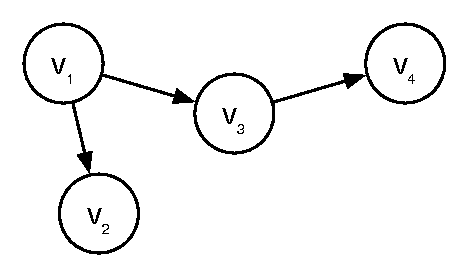
\includegraphics[scale=0.8]{img/simple-graph-example.pdf}
\caption{A simple graph.}
\label{fig: simple-example}
\end{figure}

Graphs are a natural way of expressing many problems in mathematics and computer science. They are also useful for representing programs internally in a compiler. One of the seminal graph representations is the Control Flow Graph (CFG), which was introduced by Allen \cite{808479} to explicitly represent possible control paths in a program. In the CFG, vertices are called basic blocks and contain straight-line instructions. When control enters a basic block, all instructions must be executed in that block. The edges that connect basic blocks together represent transfer of the control flow. An illustration of a CFG can be seen in Figure~\ref{fig: example-cfg}, showing a translation between some three-address code and the resulting graph. The CFG is used to convert a program into SSA form \cite{115320}. Additionally, representing a program in this way makes a number of operations simpler to perform, such as identifying loops, discovering irreducibility and performing interval analysis techniques.

\begin{figure}[ht]
\centering
\subfigure{
	\begin{minipage}[b]{0.3\linewidth}
	\texttt{\begin{tabbing}
	1: \=a = 0; \\
	\> b = 0; \\
	2: \> if x $>=$ y goto 4 \\
	3: \> a = x; \\
	\> goto 5; \\
	4: \> a = y; \\
	5: \> if a $>=$ y goto 6 \\
	\> a = a * x;\\
	\> a = a + b;\\
	\> b = b + 1;\\
	\> goto 5; \\
	6: \> ret a + b; \\
	\end{tabbing}}
	\end{minipage}
}
\subfigure{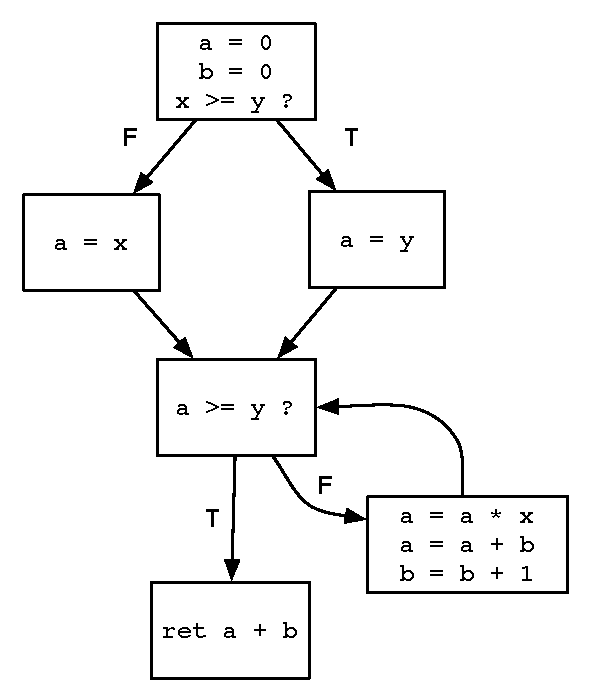
\includegraphics[scale=0.55]{img/cfg-example.pdf}}
\caption{Some three address code and the resulting CFG after translation.}
\label{fig: example-cfg}
\end{figure}

The CFG is only one example of many existing program graphs. In this section we are concerned with those that are based on SSA concepts, whether explicitly or implicitly.

\section{The SSA Graph}

We begin our exploration of graph-based SSA extensions with a very literal translation of SSA into a graph. An SSA Graph consists of vertices which represent operations, such as \texttt{add}, \texttt{load} and $\mathtt{\phi}$, and edges which determine the transfer of data through the program. For example, the incoming edges to a vertex represent the arguments required for that operation. The outgoing edge from a vertex represents the propagation of that operation's result after it has been computed. An SSA Graph $G_{SSA}=(V,E)$ consists of a set of vertices $V$ represented by tuples, and a set $E$ of edges connecting these tuples. The tuples are of the following form: 

\begin{quote}
\centering
$\langle op,left,right,ssalink\rangle$
\end{quote}

where $op$ is the unique code for the operation and $left$ and $right$ are pointers to the tuples which are the operands to this operation. Both $left$ and $right$ may not be required if a node represents a unary operation. The $ssalink$ is a pointer to the reaching definition of the variable referenced in the tuple and is used for load and store operations. Thus, we can say that this is a \textit{demand-based} graph representation. In order to compute a node, we must \text{demand} the results of the operands and then perform the computation. We show some sample SSA code translated into an SSA Graph in Figure~\ref{fig: simple-ssa-graph}.

\begin{figure}
\label{fig: simple-ssa-graph}
\caption{Some sample SSA code translated into an SSA Graph.}
\end{figure}

% =================
% Abstract is below here.
% =================

\section*{Abstract}

\subsection*{Introduction}

This chapter will explore some approaches to using SSA concepts in graph-based intermediate representations. I'm leaving the abstract here for the time being.

\subsection*{Cliff Click's simple IR}

Click and Paleczny  \cite{202534} present a simple intermediate representation which is built from SSA form. This representation shows how SSA form can be transformed into a data flow graph, using $\phi$ nodes to represent data merges. Some simple examples are given that illustrate the main concepts, and results of the authors' implementation are given.

\subsection*{The gating function}

One problem with SSA is the difficulty of directly interpreting $\phi$-functions as there is no way to explicitly tell at compile-time which of the $\phi$-variables will be chosen. This introduces the idea of the gating function -- called the $\gamma$-node -- which was introduced by Tu and Padua \cite{207115} and used by Ballance et al. in the Program Dependence Web\cite{93578} representation. We give some examples for explanation of $\phi$-translation, showing how it translates $\phi$-functions into $\gamma$-nodes.

\subsection*{Gated Single Assignment}

We then explore Havlak's work\cite{Havlak93constructionof} on Thinned Gated Single Assignment (TGSA), which is an extension of SSA with the aforementioned $\gamma$-nodes to represent a notion of control over value merges. We give some construction examples and show how loops are handled with $\mu$ and $\eta$ style representations. A short summary of the results of Havlak's implementation is given which highlights how this form is beneficial in symbolic analysis.

\subsection*{Value State Dependence Graph}

The Value State Dependence Graph (VSDG) is an intermediate representation for modeling programs using data dependencies. It can be seen as a spiritual successor to the Value Dependence Graph\cite{177907}, with the addition of ``state" edges to allow only the essential sequential dependences in a program to constrain the ordering of instructions. The IR was introduced by Johnson\cite{UCAM-CL-TR-607}, with further developments by Upton\cite{upton} and Lawrence\cite{UCAM-CL-TR-705}.

We give an outline of the key features of the VSDG and show how it is implicitly in SSA form. Construction is discussed with reference to Johnson's work. We then explain how the representation lends itself well to optimizations due to the adaptable nature of the graph. Discussion then focuses on the difficulties of generating sequential code from the graph\cite{DBLP:conf/pdpta/Upton03}, and Lawrence's proposed compiler architecture. We conclude with possible directions for ongoing work with the VSDG.

\subsection*{VSDG application: Combined Code Motion and Register Allocation}

Johnson and Mycroft \cite{johnson-combined} present an algorithm which performs code motion and register allocation at the same time by using the VSDG, uniting two phases which were traditionally believed to be antagonistic. We explore this algorithm and show how it works.


